\documentclass[11pt,a4paper]{report}

\usepackage[utf8]{inputenc}
\usepackage[T1]{fontenc}
\usepackage[italian]{babel}
\usepackage{lmodern}
\usepackage[margin=2.6cm]{geometry}
\usepackage{graphicx}
\usepackage{booktabs}
\usepackage{siunitx}
\usepackage{caption}
\usepackage{xcolor}
\usepackage{microtype}
\usepackage[hidelinks]{hyperref}
\usepackage{float}
\usepackage{tabularx}

\captionsetup{font=small,labelfont=bf,width=0.92\textwidth}
\sisetup{output-decimal-marker={,},group-separator={.},group-minimum-digits=4}
\setlength{\parskip}{0.4em}
\setlength{\parindent}{0pt}
\renewcommand{\arraystretch}{1.25}

\definecolor{autoblue}{HTML}{1f5fa8}
\definecolor{partgold}{HTML}{c99a12}
\definecolor{judgegray}{HTML}{6f747b}

\begin{document}

\chapter{Efficienza di contesto: recupero dei fatti al variare del budget}
\label{ch:efficienza-contesto}

\section{La domanda}

Il confronto principale di questa tesi fissa il budget di contesto a
\num{900} parole per tutti i sistemi. A quel budget il GraphRAG utilizza in
media circa \num{36} parole per raggiungere una recall dei fatti-gold pari a
\num{1,00}, mentre il RAG testuale ne consuma quasi \num{900} per fermarsi
molto più in basso. Un revisore può legittimamente obiettare: e se questo
divario di efficienza fosse soltanto un artefatto del budget scelto?
Concedendo al RAG testuale più contesto, il divario si chiuderebbe?

Questo capitolo risponde variando il budget su dodici livelli, da \num{100} a
\num{2400} parole, e misurando come degrada il recupero dei fatti a ciascun
livello.

\section{Metrica e metodo}

La metrica è la \textbf{recall dei fatti-gold effettivamente presenti nel
contesto} assemblato: quanta parte delle entità della risposta corretta il
sistema riesce a portare sotto gli occhi del lettore. È una quantità
\emph{deterministica} che non dipende dal modello lettore, e questo rende lo
sweep interamente offline e riproducibile senza alcuna chiave di servizio.
Per ogni livello di budget il contesto è assemblato con la stessa procedura
del sistema principale (accumulo di passaggi finché il budget è saturo). Il
GraphRAG entra come riferimento: il suo contesto è già minimo (circa \num{36}
parole) e per costruzione insensibile al budget.

\section{Risultati}

\begin{table}[H]
\centering
\caption{Recall dei fatti-gold nel contesto assemblato, al variare del budget
di contesto. Il GraphRAG è costante a \num{1,00}; BM25 e ibrido crescono
lentamente senza mai raggiungere il tetto del grafo; il denso resta molto
in basso a ogni budget.}
\label{tab:recall-budget}
\small
\begin{tabular}{r cccc}
\toprule
Budget (parole) & GraphRAG & RAG BM25 & RAG ibrido & RAG denso \\
\midrule
100  & \textbf{1,00} & 0,54 & 0,56 & 0,14 \\
150  & \textbf{1,00} & 0,58 & 0,62 & 0,18 \\
200  & \textbf{1,00} & 0,62 & 0,66 & 0,19 \\
300  & \textbf{1,00} & 0,71 & 0,73 & 0,22 \\
450  & \textbf{1,00} & 0,77 & 0,77 & 0,25 \\
600  & \textbf{1,00} & 0,80 & 0,79 & 0,27 \\
750  & \textbf{1,00} & 0,82 & 0,80 & 0,28 \\
900 (budget tesi) & \textbf{1,00} & 0,84 & 0,83 & 0,29 \\
1100 & \textbf{1,00} & 0,86 & 0,84 & 0,31 \\
1400 & \textbf{1,00} & 0,87 & 0,85 & 0,34 \\
1800 & \textbf{1,00} & 0,89 & 0,88 & 0,36 \\
2400 & \textbf{1,00} & 0,93 & 0,89 & 0,39 \\
\bottomrule
\end{tabular}
\end{table}

\begin{table}[H]
\centering
\caption{Efficienza di contesto: parole necessarie per raggiungere una data
soglia di recall dei fatti-gold. Il denso non raggiunge nessuna delle soglie
a nessun budget testato.}
\label{tab:efficienza}
\small
\begin{tabular}{c cccc}
\toprule
Soglia di recall & GraphRAG & RAG BM25 & RAG ibrido & RAG denso \\
\midrule
$\geq 60\%$ & \textbf{36} & 144 & 112 & mai \\
$\geq 70\%$ & \textbf{36} & 251 & 226 & mai \\
$\geq 80\%$ & \textbf{36} & 575 & 690 & mai \\
\bottomrule
\end{tabular}
\end{table}

\begin{figure}[H]
\centering
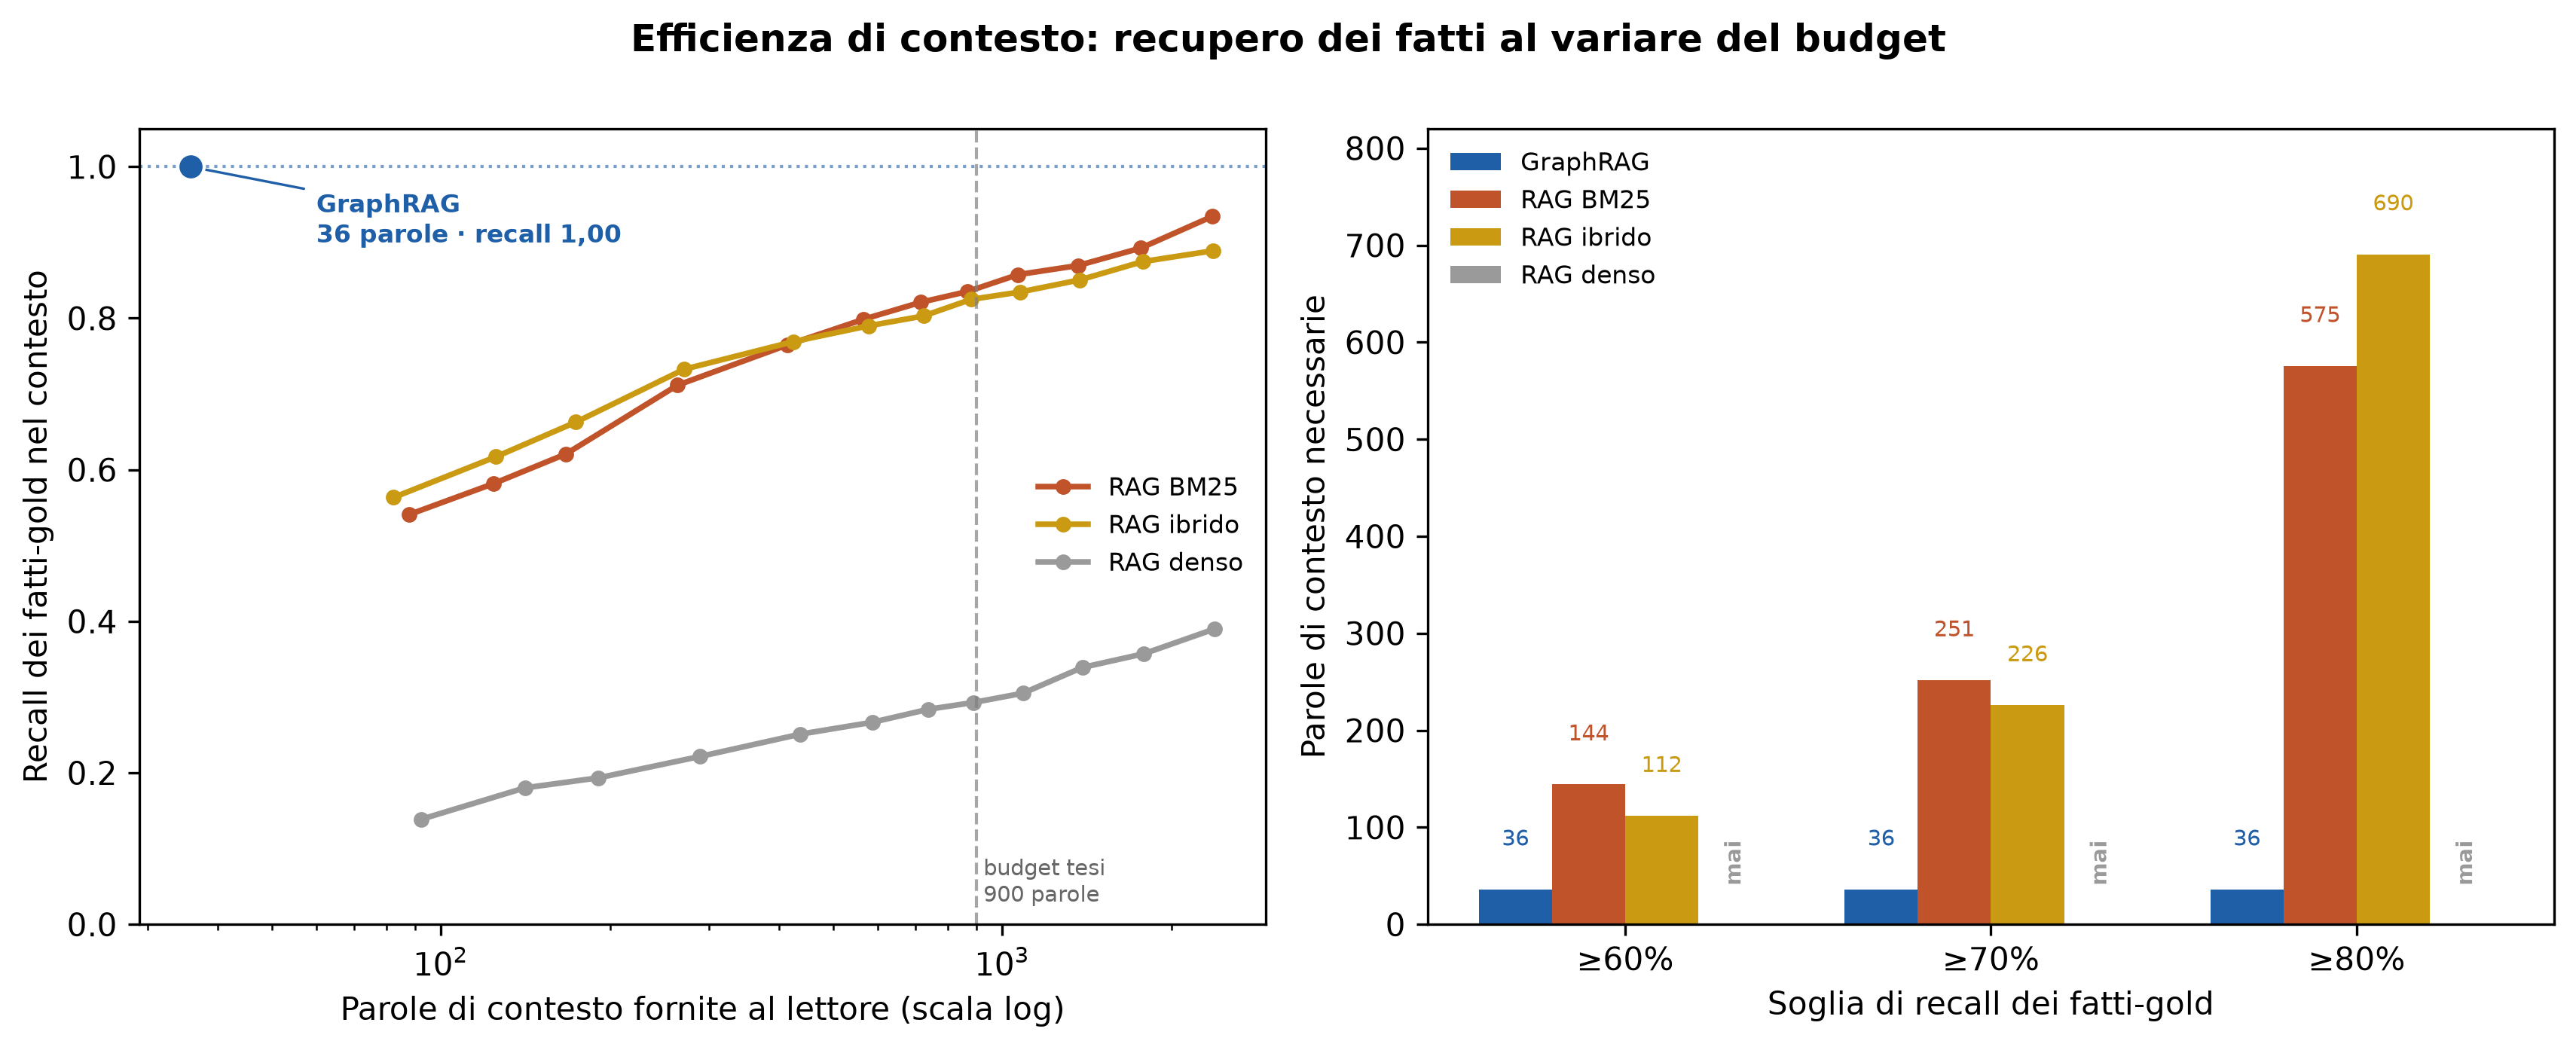
\includegraphics[width=0.98\textwidth]{fig10_context_budget.png}
\caption{Efficienza di contesto. (a) Recall dei fatti-gold in funzione delle
parole di contesto fornite al lettore (scala logaritmica): il GraphRAG è un
singolo punto in alto a sinistra (\num{36} parole, recall \num{1,00}), i RAG
testuali risalgono lentamente al crescere del contesto. (b) Parole di
contesto necessarie per raggiungere le soglie di recall del \num{60}, \num{70}
e \num{80}\%: il denso non le raggiunge mai.}
\label{fig:efficienza}
\end{figure}

\section{Interpretazione}

\textbf{Il vantaggio del GraphRAG non dipende dal budget scelto.} Anche
concedendo al RAG testuale \num{2400} parole (circa \num{2,7} volte il budget
della tesi), BM25 arriva a \num{0,93} e l'ibrido satura intorno a \num{0,89}:
nessuno dei due raggiunge il tetto del grafo (\num{1,00} con circa \num{36}
parole). Per la soglia di recall $\geq 80\%$ il GraphRAG è circa \textbf{16
volte} più efficiente di BM25 e \textbf{19 volte} più efficiente dell'ibrido.

\textbf{Il RAG denso è limitato dall'encoder, non dal contesto.} La sua
recall passa da \num{0,14} a soli \num{0,39} lungo tutto lo sweep e non
raggiunge mai neppure il \num{60}\%. Allargare il budget non lo aiuta: il
collo di bottiglia è l'encoder generico, non lo spazio di contesto. Questo
motiva, come esperimento distinto, la sostituzione con un encoder biomedico
dedicato (MedCPT, PubMedBERT, SapBERT).

\textbf{Per BM25 e ibrido il collo di bottiglia si sdoppia.} Già a \num{900}
parole la recall di retrieval (circa \num{0,83}) supera la F1 end-to-end del
lettore (circa \num{0,67} nella run principale): oltre un certo budget il
limite non è più il recupero, ma il ragionamento del lettore su un contesto
testuale lungo e rumoroso. Aggiungere parole recupera qualche fatto in più,
ma introduce anche più distrattori.

\section{Conclusione}

La curva di degrado conferma che l'efficienza di contesto del GraphRAG è una
proprietà \textbf{strutturale}, non un effetto della parametrizzazione. Il
grafo consegna al lettore esattamente i fatti-ponte richiesti in poche decine
di parole; il RAG testuale deve inondare il lettore di contesto per
avvicinarsi, senza mai raggiungere lo stesso tetto di recall. Il confronto a
\num{900} parole del capitolo principale non favorisce dunque il GraphRAG:
semmai lo penalizza, perché gli assegna un budget molto più grande di quello
che gli serve.

\end{document}
